\section{算法对照、敏感性与模型检验}
\subsection{同信息日前方法与滚动信息价值}
在相同334天、设备参数和固定电价下，DET使用前31天净负荷均值，Q80使用逐段80\%分位数，二者均调用确定性储能LP；SAA直接使用问题二，CVaR在同一历史场景上引入紧急费用尾部惩罚。上述四者在0:00拥有相同历史信息。SAA-MPC使用问题三的已发布光伏预报及日内更新，因此在表中单列为信息与机制拓展，不能用其差异证明纯算法优势。

\begin{table}[H]\centering\small
\caption{预设主方法的费用与风险比较}
\begin{tabular}{lrrrr}\toprule
方法 & 总费用/万元 & 紧急电量/万kWh & 紧急天数 & 日费CVaR95/元\\\midrule
DET & 2507.3342 & 325.7900 & 287 & 141532.0334\\
Q80 & 1773.5842 & 53.7269 & 249 & 85423.1426\\
SAA & 1760.9792 & 47.7446 & 249 & 82240.4284\\
CVaR95-L50 & 1765.8749 & 18.7619 & 248 & 67777.8076\\
SAA-MPC & 1702.0307 & 28.2086 & 243 & 74761.1946\\
\bottomrule\end{tabular}\end{table}
在预设静态主比较中，SAA的实际费用最低；Q80比SAA高约0.716\%，说明较高分位数虽然有经济解释，仍不能替代跨时段联合优化。DET的补购费用较大，反映均值计划难以应对非对称缺口损失。SAA-MPC比SAA降低费用约3.347\%，收益来源的进一步分解见第三问。

\subsection{CVaR风险规避与参数敏感性}
设历史场景全天紧急费用为$L_s=\sum_t5p_tU_t^{(s)}$，引入阈值$z$和超额损失$\xi_s$：
\begin{align}
\operatorname{CVaR}_{\alpha}(L)&=z+\frac{1}{1-\alpha}\sum_s\pi_s\xi_s,\\
\xi_s&\geq L_s-z,\quad\xi_s\geq0.
\end{align}
目标为计划费加$(1-\lambda)\mathbb E[L]+\lambda\operatorname{CVaR}_{\alpha}(L)$和微小吞吐惩罚；$z$不限制符号。预设主参数为$\alpha=0.95,\lambda=0.50$，$\lambda=0$退化为SAA。优化对象是紧急费用，表中的“日费CVaR95”则为执行后实际总费用的尾部统计，二者不可混淆。

主CVaR相对SAA增加总费用约0.278\%，紧急电量减少60.704\%，日费用CVaR95下降17.586\%，体现用较高合同费用换取尾部风险降低。经验日费CVaR95按最差5\%概率质量加权，334天对应16.7天，边界样本只取剩余权重。

\begin{table}[H]\centering\small
\caption{CVaR参数敏感性：334天实际运行指标}
\begin{tabular}{lrrrr}\toprule
$\alpha$ & $\lambda$ & 总费/万元 & 紧急量/万kWh & 日费CVaR95/元\\\midrule
0.9 & 0.25 & 1750.8386 & 25.9928 & 71450.2527\\
0.9 & 0.5 & 1763.1254 & 20.1984 & 69177.9534\\
0.9 & 0.75 & 1775.1993 & 15.5810 & 67314.8892\\
0.9 & 1.0 & 1781.5115 & 14.2774 & 67171.0438\\
0.95 & 0.25 & 1752.7502 & 24.8635 & 69870.0809\\
0.95 & 0.5 & 1765.8749 & 18.7619 & 67777.8076\\
0.95 & 0.75 & 1775.1993 & 15.5810 & 67314.8892\\
0.95 & 1.0 & 1781.5115 & 14.2774 & 67171.0438\\
0.99 & 0.25 & 1752.0906 & 24.4162 & 69300.1261\\
0.99 & 0.5 & 1765.8084 & 18.7440 & 67767.8871\\
0.99 & 0.75 & 1775.1339 & 15.5561 & 67266.2923\\
0.99 & 1.0 & 1781.4634 & 14.2596 & 67166.7326\\
\bottomrule\end{tabular}\end{table}
12组参数预先固定，用于展示权衡而不根据全年结果重新挑选主参数。其中存在费用低于SAA的组合，因此不能宣称SAA优于所有风险规避参数。31个等权场景下，$\alpha=0.99$的尾部不足一个完整场景，其CVaR等于样本最大损失；高置信度并不意味着拥有充分的极端事件信息。样本外实际费用也无需随风险权重单调变化。

\begin{figure}[H]\centering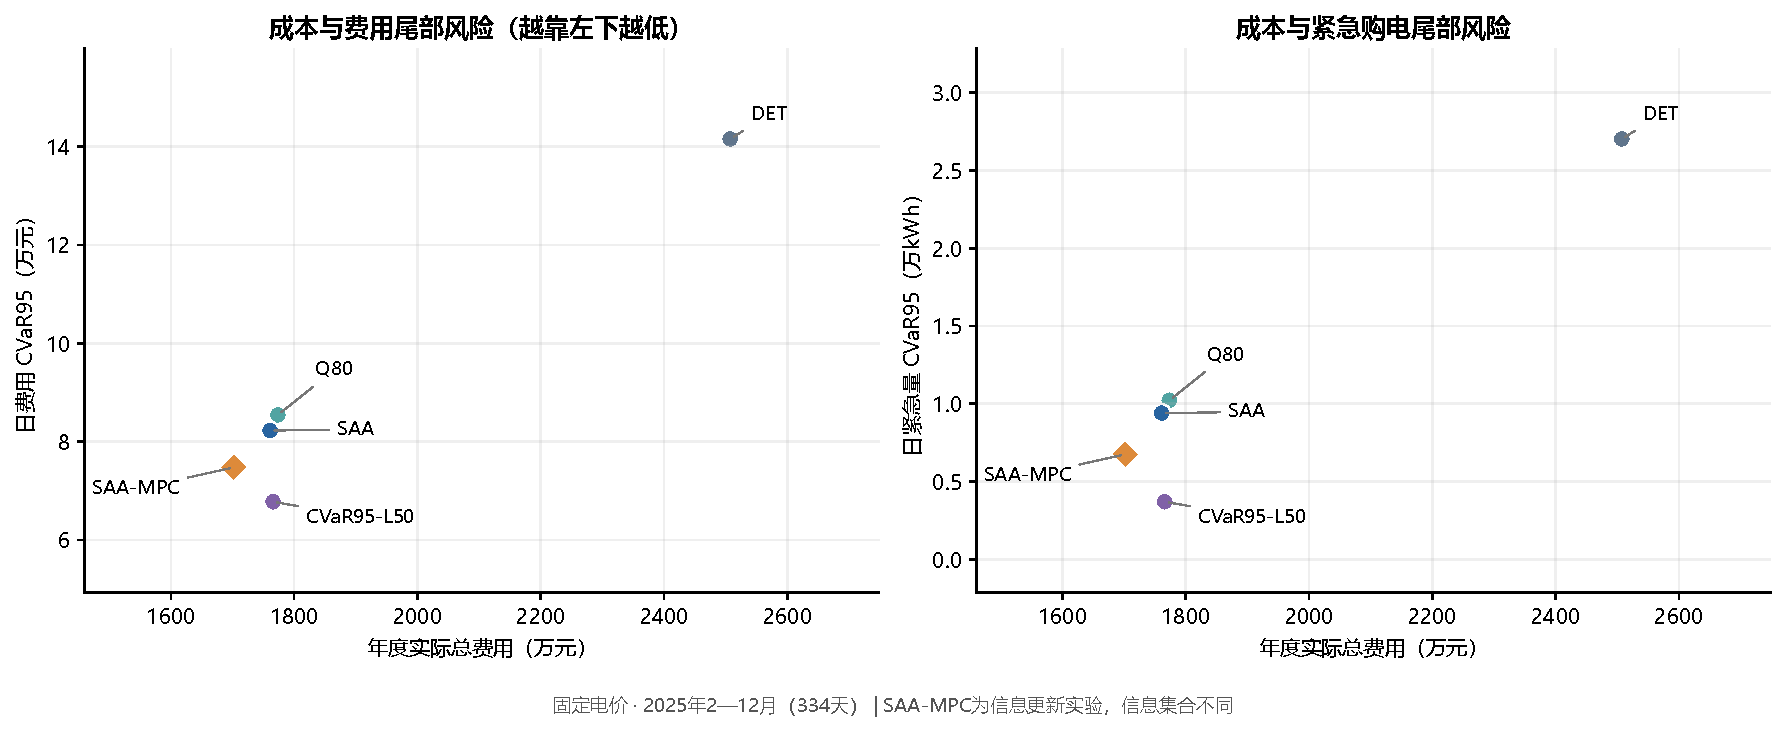
\includegraphics[width=.94\textwidth]{figures/risk_return.pdf}
\caption{预设方法的实际费用与尾部风险；MPC包含额外信息}\end{figure}
\subsection{可行性、结算与复现检验}

\begin{table}[H]\centering\small
\caption{本次合并核验的最大绝对残差（kWh）}
\begin{tabular}{lrrrr}\toprule
模型 & 供需平衡 & 储能转移 & 首末边界 & 同时充放电时段\\\midrule
Q2 & 1.14e-13 & 5.78e-12 & 0.00e+00 & 0\\
Q3 & 1.14e-13 & 1.02e-12 & 0.00e+00 & 0\\
Q4-2 & 1.14e-13 & 1.02e-12 & 0.00e+00 & 0\\
Q4-3 & 1.14e-13 & 1.02e-12 & 0.00e+00 & 0\\
\bottomrule\end{tabular}\end{table}
本次核验重算第一问和第二问334天，对第三问全期存档检查物理约束、合同恒等式及结算，并独立重算四个指定日期；第四问核对全部存档及原始价格快照。年度工作簿逐时计划、执行合同、四小时储能汇总、紧急区间与日费用均作核对。不同求解器版本可能返回等价最优解；对第二问出现差异的日期固定正式合同及四小时储能汇总重求解，核对其可行性与原最优目标，而不以新数组覆盖正式结果。

第三问19项现有测试通过，覆盖中点插值、未来实际与未发布预报隔离、执行冻结、SOC衔接、退款结算和结果导出。算法对比及12组敏感性使用归档实验结果\cite{experiment}，本次不冒称重新运行全部敏感性实验。单次运行耗时受环境影响，不作为跨硬件性能保证。

\section{模型评价与结论}
\subsection{模型优点与局限}
模型以共同线性储能约束贯穿四问，场景与真实结算分离，逐次合同调整与已执行SOC衔接清楚，便于复现及定位信息价值。正文同时给出指定日期、全期和风险对照，避免只用少量典型日支持总体结论。

局限在于：每日固定边界限制跨日调度；31天等权窗口对快速变化和尾部风险覆盖有限；未考虑电池退化、外网功率限制与未来价格预测；当前LP未显式加入互斥约束；时间标签与内部时段解释仍需最终确认。滚动求解的一系列两阶段LP不等于完整多阶段场景树，单次LP最优不代表全年实际费用全局最优。未来可引入独立验证期、季节性窗口、跨日滚动边界和电池退化成本，比较收益是否足以抵消新增复杂度。

\subsection{主要结论与运行启示}
确定性条件下，储能使示例日购电费降至35126.9486元，较无储能基准节省26.8981\%。对334天未知净负荷，SAA日前策略费用为17609791.6865元；引入光伏预报与三时刻滚动调整后为17020306.6465元，下降3.3475\%。6点与12点更新在当前回测具有明确经济收益，18点未显示额外收益。

波动电价下，4-2和4-3费用分别为17923538.0937元和17244554.4259元，同价格环境中滚动策略仍有综合经济优势。运行决策应同时关注缺口发生时刻的电价、合同富余成本与尾部风险，不能仅以平均电价、平均净负荷或最低单日费用制定策略。上述结论均限定于当前数据、价格信息假设和周期储能边界。
\FloatBarrier
